\documentclass{beamer}
 
\usepackage[utf8]{inputenc}
\usetheme{Copenhagen}


\usepackage{amsthm}
\usepackage{amsmath}
\usepackage{amssymb}
\usepackage{yfonts}
\usepackage{amssymb}
%\usepackage{fullpage}
\usepackage{mathtools}
\usepackage{tikz}
\usepackage{graphicx}
\usepackage{subcaption}
\usepackage{float}
\usepackage{pgf}
\usepackage{color}
\usepackage{hyperref}

\usetikzlibrary{arrows}

\DeclarePairedDelimiter\ceil{\lceil}{\rceil}
\DeclarePairedDelimiter\floor{\lfloor}{\rfloor}



\title{Multi-Block Analysis of the Unix crypt Cipher}
\author{Charlie Gerrie}
\institute{Dalhousie University}
\date{October 2019}
 
\usetikzlibrary{arrows}
 
\newcommand{\slide}[2]{
	\begin{frame}
		\frametitle{#1}
		#2
	\end{frame}
} 
 
 
\newcommand{\mset}[1]{\{\!\!\{#1\}\!\!\}}
\newcommand{\sigmahat}{\hat{\sigma}}
\newcommand{\conseq}{\texttt{conseq}}
\newcommand{\inv}{^{-1}}
\newcommand{\s}[1]{\{#1\}}
\newcommand{\bytes}{\mathbb{Z}_{256}}
\newcommand{\coinc}[2]{\texttt{coinc}(#1;#2)}

\begin{document}

\frame{\titlepage}

\section{The Cipher}


\slide{History} {
	Unix crypt first released in 1973. 
	\begin{figure}
		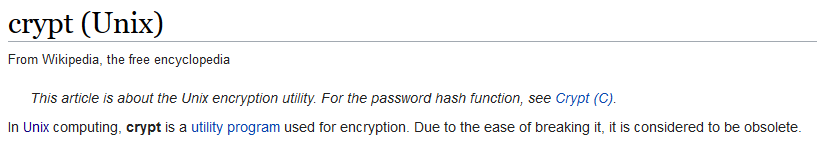
\includegraphics[width=\linewidth]{wikipedia.png}
	\end{figure}
	
}

\slide{The Key}{
	
	The key is composed of two permutations acting on the integers modulo 256. The first, $\sigma$ is fixed-point free and self-inverse, and the second, $\tau$ is a 256-cycle.
	
	\begin{figure}[H]
		\centering
		\begin{subfigure}[b]{0.45\linewidth}
		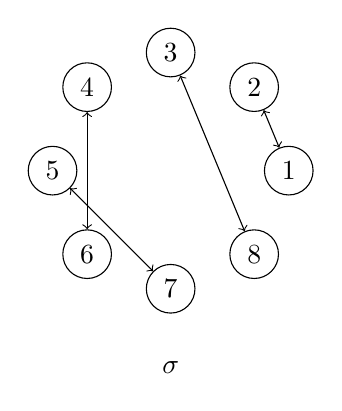
\begin{tikzpicture}[node distance=10pt]
			\foreach \i in {1,...,8} {
				\pgfmathtruncatemacro{\th}{(\i - 1) * 45}
				\node[circle,draw=black] (T\i) at (\th:1.5) {\i};
			}
			\draw[<->] (T1) -- (T2);
			\draw[<->] (T3) -- (T8);
			\draw[<->] (T4) -- (T6);
			\draw[<->] (T5) -- (T7);
			\node (title) at (270:2.5) {$\sigma$};
		\end{tikzpicture}
		\end{subfigure}
		\hfill
		\begin{subfigure}[b]{0.45\linewidth}
		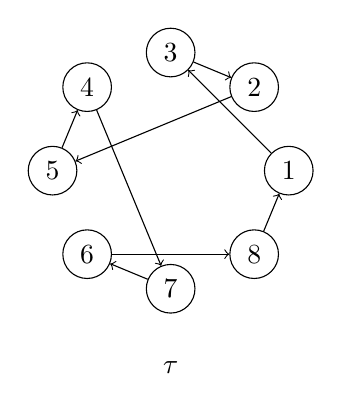
\begin{tikzpicture}[node distance=10pt]
			\foreach \i in {1,...,8} {
				\pgfmathtruncatemacro{\th}{(\i - 1) * 45}
				\node[circle,draw=black] (T\i) at (\th:1.5) {\i};
			}
			\node (title) at (270:2.5) {$\tau$};
			\draw[->] (T1) -- (T3);
			\draw[->] (T3) -- (T2);
			\draw[->] (T2) -- (T5);
			\draw[->] (T5) -- (T4);
			\draw[->] (T4) -- (T7);
			\draw[->] (T7) -- (T6);
			\draw[->] (T6) -- (T8);
			\draw[->] (T8) -- (T1);
		\end{tikzpicture}
		\end{subfigure}
	\end{figure}
}
% TODO LARGER ARROWHEADS

\slide{The Key}{
	
	The key is composed of two permutations acting on the integers modulo 256. The first, $\sigma$ is fixed-point free and self-inverse, and the second, $\tau$ is a 256-cycle.
	
	\begin{figure}[H]
		\centering
		\begin{subfigure}[b]{0.45\linewidth}
		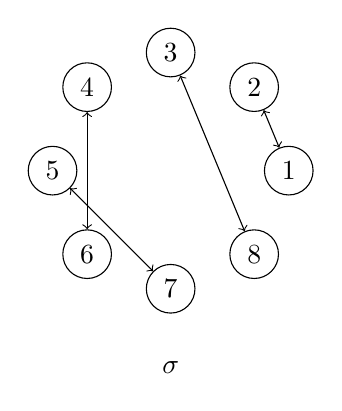
\begin{tikzpicture}[node distance=10pt]
			\foreach \i in {1,...,8} {
				\pgfmathtruncatemacro{\th}{(\i - 1) * 45}
				\node[circle,draw=black] (T\i) at (\th:1.5) {\i};
			}
			\draw[<->] (T1) -- (T2);
			\draw[<->] (T3) -- (T8);
			\draw[<->] (T4) -- (T6);
			\draw[<->] (T5) -- (T7);
			\node (title) at (270:2.5) {$\sigma$};
		\end{tikzpicture}
		\end{subfigure}
		\hfill
		\begin{subfigure}[b]{0.45\linewidth}
		\[\sigma(x)\neq x\]
		\[\sigma^2 = 1\]
		\\
		\\
		\\
		\end{subfigure}
	\end{figure}
}

\slide{The Key}{
	
	The key is composed of two permutations acting on the integers modulo 256. The first, $\sigma$ is fixed-point free and self-inverse, and the second, $\tau$ is a 256-cycle.
	
	\begin{figure}[H]
		\centering
		\begin{subfigure}[b]{0.45\linewidth}
		\[\texttt{Ord}\tau=256\]
		\\
		\\
		\\
		\\
		\end{subfigure}
		\hfill
		\begin{subfigure}[b]{0.45\linewidth}
		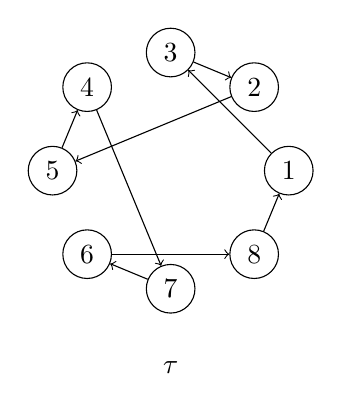
\begin{tikzpicture}[node distance=10pt]
			\foreach \i in {1,...,8} {
				\pgfmathtruncatemacro{\th}{(\i - 1) * 45}
				\node[circle,draw=black] (T\i) at (\th:1.5) {\i};
			}
			\node (title) at (270:2.5) {$\tau$};
			\draw[->] (T1) -- (T3);
			\draw[->] (T3) -- (T2);
			\draw[->] (T2) -- (T5);
			\draw[->] (T5) -- (T4);
			\draw[->] (T4) -- (T7);
			\draw[->] (T7) -- (T6);
			\draw[->] (T6) -- (T8);
			\draw[->] (T8) -- (T1);
		\end{tikzpicture}
		\end{subfigure}
	\end{figure}
}

\slide{Encoding}{
	\begin{itemize}
	
	\item Let $i=256j+k$	
	
	\item We can then encode $p_i$ into the $i$th character of the ciphertext using this equation:
%\begin{equation}
%	\label{ciphereq}

\[	c_i = \kappa^{-k} \tau^{-j} \sigma \tau^j \kappa^k p_i
\]
%\end{equation}
	where $\kappa$ is the successor function $\kappa(x)=x+1\mod 256 $.
	\end{itemize}
}

\slide{Rotary Cipher} {
	\[
	\begin{split}
		c_i =& \kappa^{-k} \tau^{-j} \sigma \tau^j \kappa^k p_i \\
		 =& \kappa^{-k} (\rho^{-1} \kappa^{-j} \rho ) (\rho^{-1} \pi \rho ) (\rho^{-1} \kappa^j \rho ) \kappa^k p_i \\
		=& \kappa^{-k} \rho^{-1} (\kappa^{-j}  \pi  \kappa^j) \rho  \kappa^k p_i
	\end{split}
	\]
}

\slide{Rotary Cipher}{
	\begin{figure}
		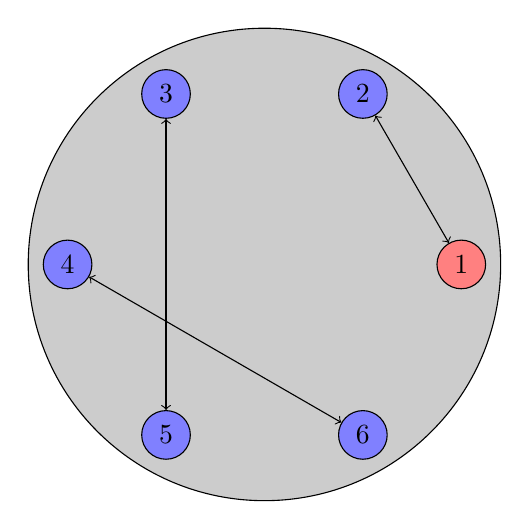
\begin{tikzpicture}[node distance=10pt]
			\filldraw[fill=black!20] (0,0) circle [radius=3];
			
			% rho
			\node[circle,draw=black,fill=red!50] (T1) at (0:2.5) {1};
			\foreach \i in {2,...,6} {
				\pgfmathtruncatemacro{\th}{(\i - 1) * 60}
				\node[circle,draw=black,fill=blue!50] (T\i) at (\th:2.5) {\i};
			}
			\draw[<->] (T1) -- (T2);
			\draw[<->] (T3) -- (T5);
			\draw[<->] (T4) -- (T6);
			
		\end{tikzpicture}
	\end{figure}
}

\slide{Rotary Cipher}{
	\begin{figure}
		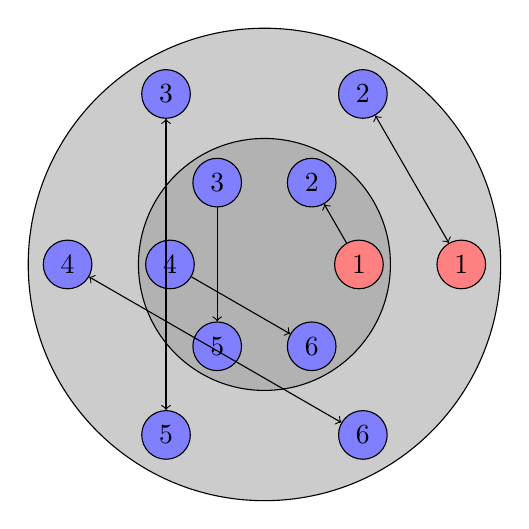
\begin{tikzpicture}[node distance=10pt]
			\filldraw[fill=black!20] (0,0) circle [radius=3];
			\filldraw[fill=black!30] (0,0) circle [radius=1.6];
			
			% pi
			
			\node[circle,draw=black,fill=red!50] (S1) at (0:1.2) {1};
			\foreach \i in {2,...,6} {
				\pgfmathtruncatemacro{\th}{(\i - 1) * 60}
				\node[circle,draw=black,fill=blue!50] (S\i) at (\th:1.2) {\i};
			}
			\draw[->] (S1) -- (S2);
			\draw[->] (S4) -- (S6);
			\draw[->] (S3) -- (S5);
			
			% rho
			
			\node[circle,draw=black,fill=red!50] (T1) at (0:2.5) {1};
			\foreach \i in {2,...,6} {
				\pgfmathtruncatemacro{\th}{(\i - 1) * 60}
				\node[circle,draw=black,fill=blue!50] (T\i) at (\th:2.5) {\i};
			}
			\draw[<->] (T1) -- (T2);
			\draw[<->] (T3) -- (T5);
			\draw[<->] (T4) -- (T6);
			
		\end{tikzpicture}
	\end{figure}
}
\slide{Rotary Cipher}{
	\begin{figure}
		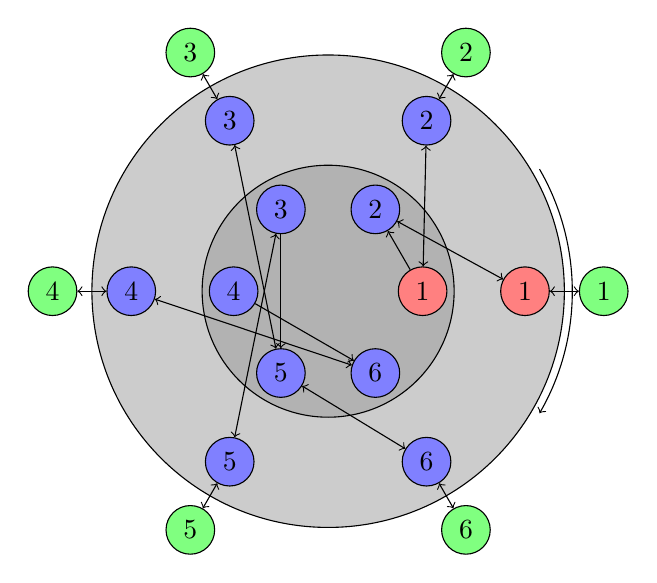
\begin{tikzpicture}[node distance=10pt]
			\filldraw[fill=black!20] (0,0) circle [radius=3];
			\filldraw[fill=black!30] (0,0) circle [radius=1.6];
			
			% pi
			
			\node[circle,draw=black,fill=red!50] (S1) at (0:1.2) {1};
			\foreach \i in {2,...,6} {
				\pgfmathtruncatemacro{\th}{(\i - 1) * 60}
				\node[circle,draw=black,fill=blue!50] (S\i) at (\th:1.2) {\i};
			}
			\draw[->] (S1) -- (S2);
			\draw[->] (S4) -- (S6);
			\draw[->] (S3) -- (S5);
			
			% rho
			
			\node[circle,draw=black,fill=red!50] (T1) at (0:2.5) {1};
			\foreach \i in {2,...,6} {
				\pgfmathtruncatemacro{\th}{(\i - 1) * 60}
				\node[circle,draw=black,fill=blue!50] (T\i) at (\th:2.5) {\i};
			}
			\draw[<->] (T1) -- (S2);
			\draw[<->] (T2) -- (S1);
			\draw[<->] (T3) -- (S5);
			\draw[<->] (T5) -- (S3);
			\draw[<->] (T4) -- (S6);
			\draw[<->] (T6) -- (S5);
						
			\foreach \i in {1,...,6} {
			\pgfmathtruncatemacro{\th}{(\i-1) * 60}
				\node[circle,draw=black,fill=green!50] (I\i) at (\th:3.5) {\i};
			}
			\draw[<->] (I1) -- (T1);
			\draw[<->] (I2) -- (T2);
			\draw[<->] (I3) -- (T3);
			\draw[<->] (I4) -- (T4);
			\draw[<->] (I5) -- (T5);
			\draw[<->] (I6) -- (T6);
			
			\draw[<-] (-30:3.1) arc (-30:30:3.1);		
			
		\end{tikzpicture}
	\end{figure}
}
\slide{Rotary Cipher}{
	\begin{figure}
		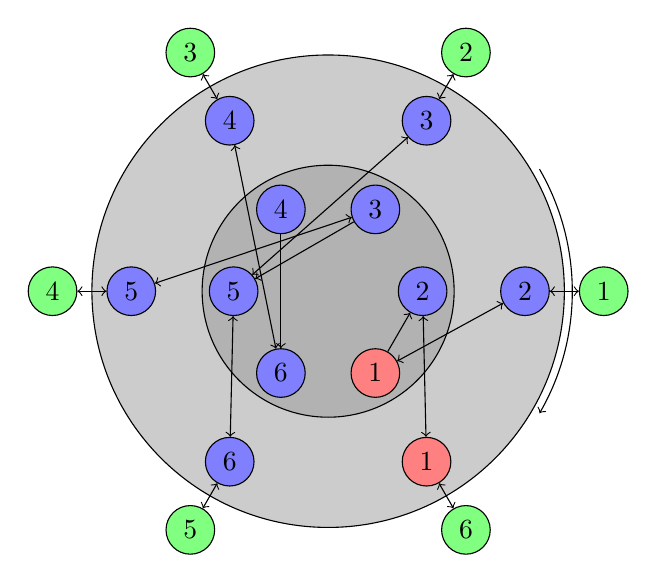
\begin{tikzpicture}[node distance=10pt]
			\filldraw[fill=black!20] (0,0) circle [radius=3];
			\filldraw[fill=black!30] (0,0) circle [radius=1.6];
			
			% pi
			
			\node[circle,draw=black,fill=red!50] (S1) at (-60:1.2) {1};
			\foreach \i in {2,...,6} {
				\pgfmathtruncatemacro{\th}{(\i-2) * 60}
				\node[circle,draw=black,fill=blue!50] (S\i) at (\th:1.2) {\i};
			}
			\draw[->] (S1) -- (S2);
			\draw[->] (S4) -- (S6);
			\draw[->] (S3) -- (S5);
			
			% rho
			
			\node[circle,draw=black,fill=red!50] (T1) at (-60:2.5) {1};
			\foreach \i in {2,...,6} {
				\pgfmathtruncatemacro{\th}{(\i-2) * 60}
				\node[circle,draw=black,fill=blue!50] (T\i) at (\th:2.5) {\i};
			}
			\draw[<->] (T1) -- (S2);
			\draw[<->] (T2) -- (S1);
			\draw[<->] (T3) -- (S5);
			\draw[<->] (T5) -- (S3);
			\draw[<->] (T4) -- (S6);
			\draw[<->] (T6) -- (S5);
			
			\foreach \i in {1,...,6} {
			\pgfmathtruncatemacro{\th}{(\i-1) * 60}
				\node[circle,draw=black,fill=green!50] (I\i) at (\th:3.5) {\i};
			}
			\draw[<->] (I1) -- (T2);
			\draw[<->] (I2) -- (T3);
			\draw[<->] (I3) -- (T4);
			\draw[<->] (I4) -- (T5);
			\draw[<->] (I5) -- (T6);
			\draw[<->] (I6) -- (T1);
			
			\draw[<-] (-30:3.1) arc (-30:30:3.1);	
			
		\end{tikzpicture}
	\end{figure}
}
\slide{Rotary Cipher}{
	\begin{figure}
		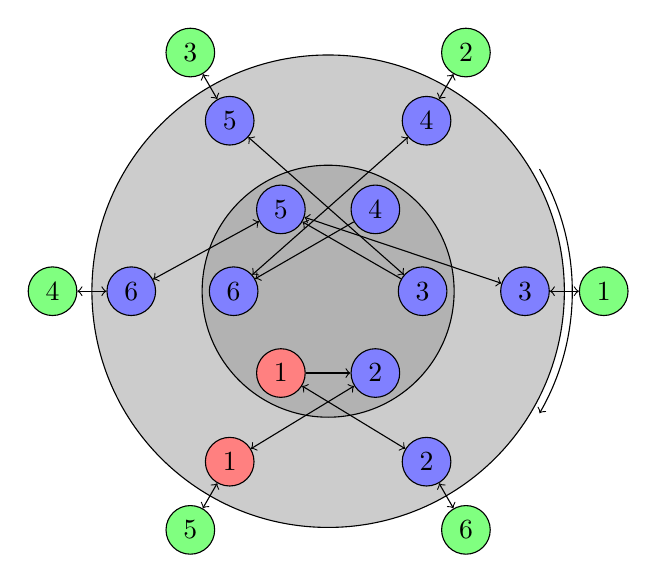
\begin{tikzpicture}[node distance=10pt]
			\filldraw[fill=black!20] (0,0) circle [radius=3];
			\filldraw[fill=black!30] (0,0) circle [radius=1.6];
			
			% pi
			
			\node[circle,draw=black,fill=red!50] (S1) at (-120:1.2) {1};
			\foreach \i in {2,...,6} {
				\pgfmathtruncatemacro{\th}{(\i-3) * 60}
				\node[circle,draw=black,fill=blue!50] (S\i) at (\th:1.2) {\i};
			}
			\draw[->] (S1) -- (S2);
			\draw[->] (S4) -- (S6);
			\draw[->] (S3) -- (S5);
			
			% rho
			
			\node[circle,draw=black,fill=red!50] (T1) at (-120:2.5) {1};
			\foreach \i in {2,...,6} {
				\pgfmathtruncatemacro{\th}{(\i-3) * 60}
				\node[circle,draw=black,fill=blue!50] (T\i) at (\th:2.5) {\i};
			}
			\draw[<->] (T1) -- (S2);
			\draw[<->] (T2) -- (S1);
			\draw[<->] (T3) -- (S5);
			\draw[<->] (T5) -- (S3);
			\draw[<->] (T4) -- (S6);
			\draw[<->] (T6) -- (S5);
			
			\foreach \i in {1,...,6} {
			\pgfmathtruncatemacro{\th}{(\i-1) * 60}
				\node[circle,draw=black,fill=green!50] (I\i) at (\th:3.5) {\i};
			}
			\draw[<->] (I1) -- (T3);
			\draw[<->] (I2) -- (T4);
			\draw[<->] (I3) -- (T5);
			\draw[<->] (I4) -- (T6);
			\draw[<->] (I5) -- (T1);
			\draw[<->] (I6) -- (T2);
			
			\draw[<-] (-30:3.1) arc (-30:30:3.1);	
		\end{tikzpicture}
	\end{figure}
}
\slide{Rotary Cipher}{
	\begin{figure}
		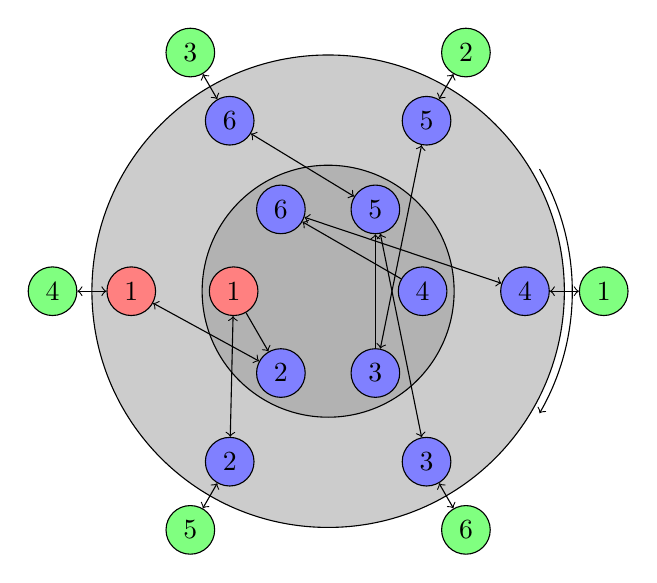
\begin{tikzpicture}[node distance=10pt]
			\filldraw[fill=black!20] (0,0) circle [radius=3];
			\filldraw[fill=black!30] (0,0) circle [radius=1.6];
			
			% pi
			
			\node[circle,draw=black,fill=red!50] (S1) at (-180:1.2) {1};
			\foreach \i in {2,...,6} {
				\pgfmathtruncatemacro{\th}{(\i-4) * 60}
				\node[circle,draw=black,fill=blue!50] (S\i) at (\th:1.2) {\i};
			}
			\draw[->] (S1) -- (S2);
			\draw[->] (S4) -- (S6);
			\draw[->] (S3) -- (S5);
			
			% rho
			
			\node[circle,draw=black,fill=red!50] (T1) at (-180:2.5) {1};
			\foreach \i in {2,...,6} {
				\pgfmathtruncatemacro{\th}{(\i-4) * 60}
				\node[circle,draw=black,fill=blue!50] (T\i) at (\th:2.5) {\i};
			}
			\draw[<->] (T1) -- (S2);
			\draw[<->] (T2) -- (S1);
			\draw[<->] (T3) -- (S5);
			\draw[<->] (T5) -- (S3);
			\draw[<->] (T4) -- (S6);
			\draw[<->] (T6) -- (S5);
			
			\foreach \i in {1,...,6} {
			\pgfmathtruncatemacro{\th}{(\i-1) * 60}
				\node[circle,draw=black,fill=green!50] (I\i) at (\th:3.5) {\i};
			}
			\draw[<->] (I1) -- (T4);
			\draw[<->] (I2) -- (T5);
			\draw[<->] (I3) -- (T6);
			\draw[<->] (I4) -- (T1);
			\draw[<->] (I5) -- (T2);
			\draw[<->] (I6) -- (T3);
			
			\draw[<-] (-30:3.1) arc (-30:30:3.1);	
		\end{tikzpicture}
	\end{figure}
}
\slide{Rotary Cipher}{
	\begin{figure}
		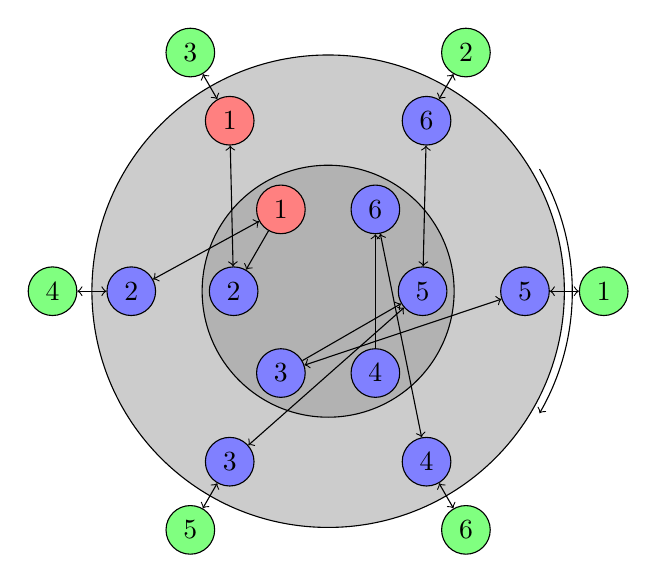
\begin{tikzpicture}[node distance=10pt]
			\filldraw[fill=black!20] (0,0) circle [radius=3];
			\filldraw[fill=black!30] (0,0) circle [radius=1.6];
			
			% pi
			
			\node[circle,draw=black,fill=red!50] (S1) at (-240:1.2) {1};
			\foreach \i in {2,...,6} {
				\pgfmathtruncatemacro{\th}{(\i-5) * 60}
				\node[circle,draw=black,fill=blue!50] (S\i) at (\th:1.2) {\i};
			}
			\draw[->] (S1) -- (S2);
			\draw[->] (S4) -- (S6);
			\draw[->] (S3) -- (S5);
			
			% rho
			
			\node[circle,draw=black,fill=red!50] (T1) at (-240:2.5) {1};
			\foreach \i in {2,...,6} {
				\pgfmathtruncatemacro{\th}{(\i-5) * 60}
				\node[circle,draw=black,fill=blue!50] (T\i) at (\th:2.5) {\i};
			}
			\draw[<->] (T1) -- (S2);
			\draw[<->] (T2) -- (S1);
			\draw[<->] (T3) -- (S5);
			\draw[<->] (T5) -- (S3);
			\draw[<->] (T4) -- (S6);
			\draw[<->] (T6) -- (S5);
			
			\foreach \i in {1,...,6} {
			\pgfmathtruncatemacro{\th}{(\i-1) * 60}
				\node[circle,draw=black,fill=green!50] (I\i) at (\th:3.5) {\i};
			}
			\draw[<->] (I1) -- (T5);
			\draw[<->] (I2) -- (T6);
			\draw[<->] (I3) -- (T1);
			\draw[<->] (I4) -- (T2);
			\draw[<->] (I5) -- (T3);
			\draw[<->] (I6) -- (T4);
			
			\draw[<-] (-30:3.1) arc (-30:30:3.1);	
		\end{tikzpicture}
	\end{figure}
}
\slide{Rotary Cipher}{
	\begin{figure}
		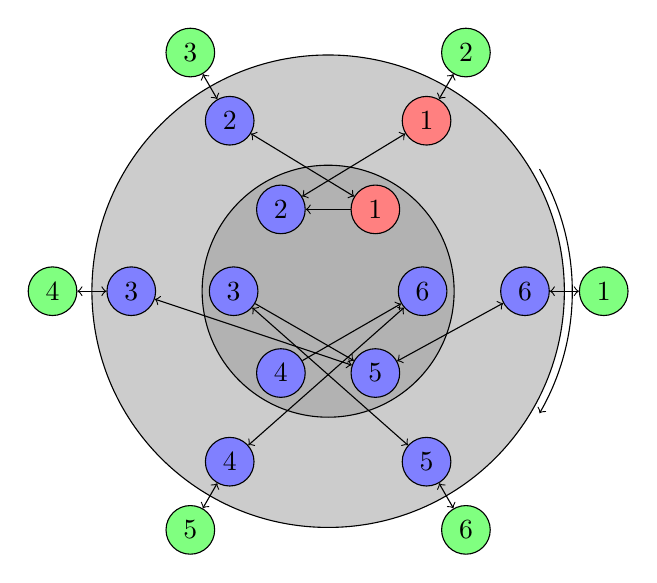
\begin{tikzpicture}[node distance=10pt]
			\filldraw[fill=black!20] (0,0) circle [radius=3];
			\filldraw[fill=black!30] (0,0) circle [radius=1.6];
			
			% pi
			
			\node[circle,draw=black,fill=red!50] (S1) at (-300:1.2) {1};
			\foreach \i in {2,...,6} {
				\pgfmathtruncatemacro{\th}{(\i-6) * 60}
				\node[circle,draw=black,fill=blue!50] (S\i) at (\th:1.2) {\i};
			}
			\draw[->] (S1) -- (S2);
			\draw[->] (S4) -- (S6);
			\draw[->] (S3) -- (S5);
			
			% rho
			
			\node[circle,draw=black,fill=red!50] (T1) at (-300:2.5) {1};
			\foreach \i in {2,...,6} {
				\pgfmathtruncatemacro{\th}{(\i-6) * 60}
				\node[circle,draw=black,fill=blue!50] (T\i) at (\th:2.5) {\i};
			}
			\draw[<->] (T1) -- (S2);
			\draw[<->] (T2) -- (S1);
			\draw[<->] (T3) -- (S5);
			\draw[<->] (T5) -- (S3);
			\draw[<->] (T4) -- (S6);
			\draw[<->] (T6) -- (S5);
			
			\foreach \i in {1,...,6} {
			\pgfmathtruncatemacro{\th}{(\i-1) * 60}
				\node[circle,draw=black,fill=green!50] (I\i) at (\th:3.5) {\i};
			}
			\draw[<->] (I1) -- (T6);
			\draw[<->] (I2) -- (T1);
			\draw[<->] (I3) -- (T2);
			\draw[<->] (I4) -- (T3);
			\draw[<->] (I5) -- (T4);
			\draw[<->] (I6) -- (T5);
			
			\draw[<-] (-30:3.1) arc (-30:30:3.1);	
		\end{tikzpicture}
	\end{figure}
}
\slide{Rotary Cipher}{
	\begin{figure}
		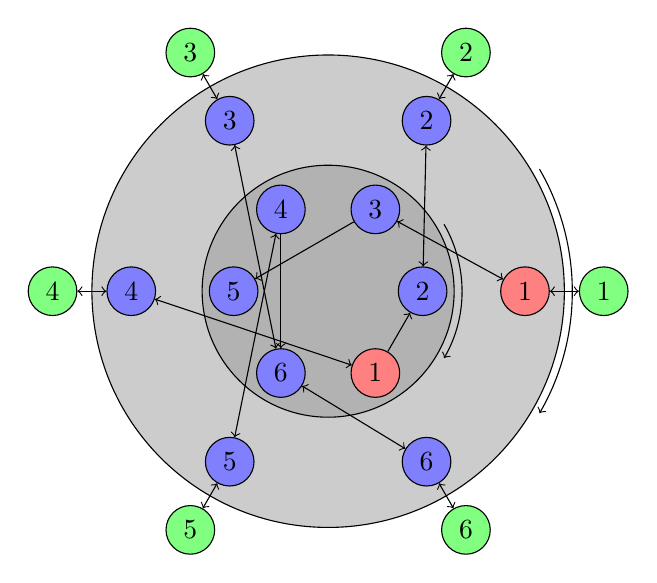
\begin{tikzpicture}[node distance=10pt]
			\filldraw[fill=black!20] (0,0) circle [radius=3];
			\filldraw[fill=black!30] (0,0) circle [radius=1.6];
			
			% pi
			
			\node[circle,draw=black,fill=red!50] (S1) at (-60:1.2) {1};
			\foreach \i in {2,...,6} {
				\pgfmathtruncatemacro{\th}{(\i-8) * 60}
				\node[circle,draw=black,fill=blue!50] (S\i) at (\th:1.2) {\i};
			}
			\draw[->] (S1) -- (S2);
			\draw[->] (S4) -- (S6);
			\draw[->] (S3) -- (S5);
			
			% rho
			
			\node[circle,draw=black,fill=red!50] (T1) at (0:2.5) {1};
			\foreach \i in {2,...,6} {
				\pgfmathtruncatemacro{\th}{(\i-7) * 60}
				\node[circle,draw=black,fill=blue!50] (T\i) at (\th:2.5) {\i};
			}
			\draw[<->] (T1) -- (S3);
			\draw[<->] (T2) -- (S2);
			\draw[<->] (T3) -- (S6);
			\draw[<->] (T5) -- (S4);
			\draw[<->] (T4) -- (S1);
			\draw[<->] (T6) -- (S6);
			
			\foreach \i in {1,...,6} {
			\pgfmathtruncatemacro{\th}{(\i-1) * 60}
				\node[circle,draw=black,fill=green!50] (I\i) at (\th:3.5) {\i};
			}
			\draw[<->] (I1) -- (T1);
			\draw[<->] (I2) -- (T2);
			\draw[<->] (I3) -- (T3);
			\draw[<->] (I4) -- (T4);
			\draw[<->] (I5) -- (T5);
			\draw[<->] (I6) -- (T6);
			
			\draw[<-] (-30:3.1) arc (-30:30:3.1);
			\draw[<-] (-30:1.7) arc (-30:30:1.7);	
		\end{tikzpicture}
	\end{figure}
}





\slide{Block Keys} {
	\begin{itemize}
	
	\item Unix crypt splits the plaintext to be encoded into blocks of 256 characters.
	
	\item
	Recall the equation for encoding the $i$th character, where $i=256j+k$:
	\[	c_i = \kappa^{-k} \tau^{-j} \sigma \tau^j \kappa^k p_i
	\]
	Notice that the power on $\tau$ only increases when $j$ does, so every 256 characters. Thus we can define the $j$th block key as:
	\[  \sigma_i = \tau^{-j} \sigma \tau^j
	\]
	\end{itemize}
}


\section{Collecting Data}
\slide{Single-block} {
	\begin{itemize}
	
	\item \textbf{The single-block analysis gives us approximations of the block keys.} 
	\item It does this by using \emph{a priori} statistics about the probabilities of different characters being in proximity to other characters.
	\item We will denote these block key approximations by $\hat{\sigma}_i$. 
	% TODO examples
	
	\end{itemize}
	
}

\slide{Multi-block plan} {
	Our plan is to take the block key approximations from the single-block analysis and "connect the dots". The hard part is reconstructing $\tau$. Once we have $\tau$ it is relatively easy to recover the other half of the key, $\sigma$.
}

\slide{Wires}{
	\begin{itemize}
	\item For a given permutation $\sigma$, a \emph{wire} is a pair $(a,b)$ such that $\sigma(a)=b$. 
	\item e.g. $(2,5)$, $(7,6)$
	\end{itemize}
	\begin{figure}
	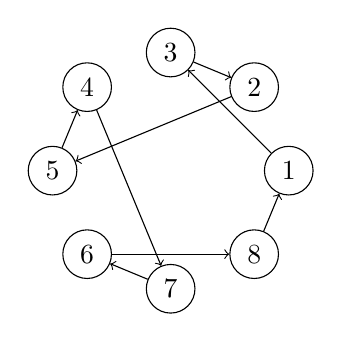
\begin{tikzpicture}[node distance=10pt]
			\foreach \i in {1,...,8} {
				\pgfmathtruncatemacro{\th}{(\i - 1) * 45}
				\node[circle,draw=black] (T\i) at (\th:1.5) {\i};
			}
			
			\draw[->] (T1) -- (T3);
			\draw[->] (T3) -- (T2);
			\draw[->] (T2) -- (T5);
			\draw[->] (T5) -- (T4);
			\draw[->] (T4) -- (T7);
			\draw[->] (T7) -- (T6);
			\draw[->] (T6) -- (T8);
			\draw[->] (T8) -- (T1);
		\end{tikzpicture}
		\end{figure}
}

\slide{Multisets}{
	\begin{itemize}
		\item A multiset $X$ of cardinality $|X|$ is the equivalence class of $|X|$-tuples up to permutations. Sorting the elements yields a unique representation.
		\item  We say an element is \emph{in} a multiset if it appears at least once in the tuple. The \emph{multiplicity} of an element is the number of times it appears in the list. 
		\item e.g. (1,1,2,2,2,3)
	\end{itemize}
	
}



\slide{Some Algebra}{
	
	\begin{figure}[H]
		\centering
		\begin{subfigure}[b]{0.6\linewidth}
		\begin{itemize}
			\item If we conjecture that $(a,b)$ is a wire in $\tau$ then it must also be a wire in $\sigma_1 \tau \sigma^{-1}_0$.
			\item But the wire in $\sigma_1 \tau \sigma^{-1}_0$ is really three wires: a wire $(a,\sigma_1(a))$ in $\sigma_1$, a wire $(\sigma_1(a),\sigma_0(b))$ in $\tau$, and a wire $(\sigma_0(b), b)$ in $\sigma^{-1}_0$. Thus, if $(a,b)$ is a wire in $\tau$ then $(\sigma_1(a),\sigma_0(b))$ must also be a wire in $\tau$. In general, all wires $(\sigma_{i+1}(a),\sigma_i(b))$ must be in $\tau$.
			\item The \emph{wire consequences} of $(a,b)$ are all the wires that must also be in $\tau$ if $(a,b)$ is.

		\end{itemize}
		\end{subfigure}
		\begin{subfigure}[b]{0.3\linewidth}
			\caption{Commutative Diagram}
			\centering
			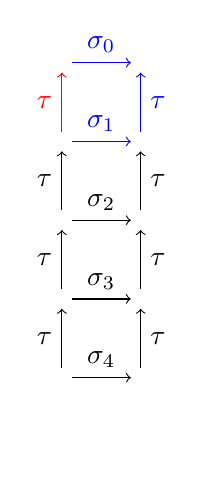
\begin{tikzpicture}[node distance=10pt]
		\foreach \i in {0,...,4} {
			\node (L\i) at (0,-\i) {};
			\node (R\i) at (1,-\i) {};
		}
		\foreach \i in {0,...,4} {
			\node (BL\i) at (0,-\i-1) {};
			\node (BR\i) at (1,-\i-1) {};
		}
		\draw [red, arrows={->}] (BL0) edge node[left] {$\tau$} (L0);
		\draw [blue, arrows={->}] (L0) edge node[above] {$\sigma_0$} (R0);
		\draw [blue, arrows={->}] (BR0) edge node[right] {$\tau$} (R0);
		\draw [blue, arrows={->}] (L1) edge node[above] {$\sigma_1$} (R1);
		\foreach \i in {2,...,4} {
			\draw [->] (L\i) edge node[above] {$\sigma_\i$} (R\i);
		}
		\foreach \i in {1,...,3} {
			\draw [->] (BL\i) edge node[left] {$\tau$} (L\i);
			\draw [->] (BR\i) edge node[right] {$\tau$} (R\i);
		}
		\end{tikzpicture}
		
		\end{subfigure}
	\end{figure}
	
}

\slide{Consequences}{
	% reference Algebra
	For a wire $(a,b)$, we have
	\begin{equation}
		\conseq(a,b)=\mset{\sigmahat_i(a), \sigmahat_{i+1}(b)) : 0\leq i<N-1}\end{equation}
	where $N$ is the number of $\sigmahat$'s. This is a multiset.
}

\slide{Coincidences}{
	We define an indicator function $\delta$ taking two arguments $x$ and $y$
\[
	\delta(x,y)=
	\begin{cases}
		1 & \texttt{if}\ x=y \\
		0 & \texttt{if}\ x \neq y
	\end{cases}
\]
Then for any two multisets $X$ and $Y$ with elements $x_i$ and $y_j$, where $0\leq i < |X|$ and $0\leq j < |Y|$, we define their \emph{coincidence} as:
\[
	\coinc{X}{Y} = \sum_{i,j} \delta(x_i,y_j)
\]
with the sum being over all possible pairs of $i$ and $j$.
}

\slide{Coincidences} {
	% particular to blocks
	If we consider two wires $(a,b)$ and $(c,d)$, then we have
	\begin{equation}
		\label{coinceq}
		\texttt{coinc}(a,b,c,d)=\sum^{255}_{i=0} \sum^{255}_{j=0} \texttt{conseq}(a,b)_{i,j} \texttt{conseq}(c,d)_{i,j}
	\end{equation}
	where $\texttt{conseq}(a,b)_{i,j}$ is the multiplicity of the wire $(i,j)$ in the consequences of $(a,b)$.
}

\slide{Coincidences} {
	\begin{figure}
		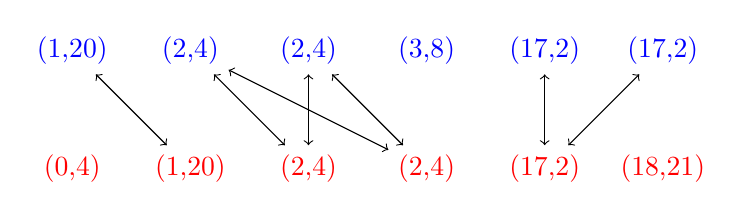
\begin{tikzpicture}
		%\node (cons1) at (-2.5,0) {$\texttt{conseq}(c,d)$};
		%\node (cons2) at (-2.5,1.5) {$\texttt{conseq}(a,b)$};	
	
		\node (T1) at (0,0) {\textcolor{red}{(0,4)}};
		\node (T2) at (1.5,0) {\textcolor{red}{(1,20)}};
		\node (T3) at (3,0) {\textcolor{red}{(2,4)}};
		\node (T4) at (4.5,0) {\textcolor{red}{(2,4)}};
		\node (T5) at (6,0) {\textcolor{red}{(17,2)}};
		\node (T6) at (7.5,0) {\textcolor{red}{(18,21)}};
		\node (B1) at (0,1.5) {\textcolor{blue}{(1,20)}};
		\node (B2) at (1.5,1.5) {\textcolor{blue}{(2,4)}};
		\node (B3) at (3,1.5) {\textcolor{blue}{(2,4)}};
		\node (B4) at (4.5,1.5) {\textcolor{blue}{(3,8)}};
		\node (B5) at (6,1.5) {\textcolor{blue}{(17,2)}};
		\node (B6) at (7.5,1.5) {\textcolor{blue}{(17,2)}};
		
		\draw [<->] (T2) -- (B1);
		\draw [<->] (T3) -- (B2);
		\draw [<->] (T4) -- (B2);
		\draw [<->] (T3) -- (B3);
		\draw [<->] (T4) -- (B3);
		\draw [<->] (T5) -- (B5);
		\draw [<->] (T5) -- (B6);
	\end{tikzpicture}
	\end{figure}
}


\section{Statistics}
\slide{Statistics}{
	Now that we can calculate the number of coincidences between the consequences of different wires, we will use statistics on this data to choose the correct wires in $\tau$.
}
\slide{A Bag Example}{
	\begin{itemize}
	\item I have two bags filled with marked balls. One has 10 balls in it, the other 100.
	
	\item Just by iteratively removing balls from the bags and examining them, how can I tell which bag has the 10 balls and which the 100?
	\end{itemize}
}

\slide{The Answer}{
	We take a ball out, remember it, and place it back in the bag. Then we take another ball and note if we drew the same ball as last time. This will happen about 10\% of the time for one bag and 1\% of the time for the other. In other words, the probability of drawing the same ball twice in a row will be distributed differently for the two bags.
}

\slide{The Null Distribution} {
	For each possible wire endpoint, we consider two hypotheses.
	\begin{enumerate}
		\item The alternative hypothesis: that this is the correct endpoint.
		\item The null hypothesis: that this is the wrong endpoint.
	\end{enumerate}
}

\slide{The Null Distribution}{
	In the null hypothesis case the endpoint is wrong. Thus none of the correlations from the conjugacies of the block keys apply, so the wires are chosen randomly.
	
	\begin{center}
\begin{tabular}{|c|c|c|c|c|}
\hline
$X$ & 0 & 1 & 2 & ... \\
\hline 
$P(\texttt{coinc}(a,b,c,d)=X)$ & 0.965 & 0.0345 & 0.000618 & ... \\

\hline
\end{tabular}
\end{center}
}

\slide{Bayes' Law}{
	 Now we have two potential distributions and we would like to know which one our sample distribution follows. Let $D_1$ and $D_2$ be the events that the sample distribution follows the two distributions and $S$ is the event of getting the samples that we did.  Normally we would then use Bayes' theorem:
\[ P(D_1 | S) = \frac{P(S | D_1) P(D_1)}{P(S)} \]
But this would require us to know an \emph{a priori} probability of the distribution and the samples. This we cannot know, so Bayes' theorem fails us. 
}
\slide{Likelihood} {
	\begin{itemize}	
	\item We will be using a concept from statistics and probability theory known as \emph{likelihood}. If we consider two events $A$ and $B$, then likelihood is related to conditional probability by the relation 
\[ \mathcal{L}(A|B)=P(B|A)\]
\item It is easy to calculate $P(S | D_1 )$ and $P(S | D_2 )$. Assuming the samples are independent, they are simply the products of the pdf values for all the samples. Thus we can acquire $\mathcal{L}(D_1 | S)$ and $\mathcal{L}(D_2 | S)$. 
	\end{itemize}
}

\slide{Likelihood} {
	\begin{itemize}
	\item Now we can apply what is known as the Maximum Likelihood Method. What this means is that rather than choosing what the most \emph{probable} wire endpoint for each wire, we choose the most \emph{likely} one.
	\item The wire most likely to be correct is the wire least likely to be incorrect i.e. follow the null distribution.
	\end{itemize}
}



\slide{Picking a wire} {
	Here are some coincidences distributions for a wire:
\begin{center}
\begin{tabular}{|c|c|c|c|c|}
\hline
$X$ & 0 & 1 & 2 & ... \\
\hline 
$P(\texttt{coinc}(15,1,c,d)=X)$ & 0.940 & 0.0580 & 0.00178 & ... \\
$P(\texttt{coinc}(15,2,c,d)=X)$ & 0.940 & 0.0583 & 0.00147 & ... \\
$P(\texttt{coinc}(15,3,c,d)=X)$ & \textcolor{red}{0.944} & \textcolor{red}{0.0515} & \textcolor{red}{0.00262} & \textcolor{red}{...} \\
$P(\texttt{coinc}(15,4,c,d)=X)$ & 0.940 & 0.0578 & 0.00167 & ... \\

\hline

\end{tabular}
\end{center}
}

\slide{Finding $\sigma$} {
	\begin{itemize}
		\item Recall that $\sigma_i = \tau^{-j} \sigma \tau^j$, so $\sigma = \tau^j \sigma_i \tau^{-j}$.
		\item Thus once we have recovered $\tau$, we can construct as many guesses at $\sigma$ as we have blocks. Then we simply pick the wires that occur in the majority of these.
	\end{itemize}
}

\slide{Conclusion}{
	Thus it is possible to algorithmically recover the key using only the ciphertext and the character-distribution data used by the single-block algorithm. Our work now is in trying to decrease the number of blocks we need to successfully recover the key. 
}

\slide{Thank you}{
	I would like to thank Peter Selinger, Dalhousie University and NSERC.
}

% LET'S GET 25 GOOD SLIDES!%

\end{document}